%\documentclass[handout]{ximera}
\documentclass[nooutcomes]{ximera}

\usepackage{gensymb}
\usepackage{tabularx}
\usepackage{mdframed}
\usepackage{pdfpages}
%\usepackage{chngcntr}

\let\problem\relax
\let\endproblem\relax

\newcommand{\property}[2]{#1#2}




\newtheoremstyle{SlantTheorem}{\topsep}{\fill}%%% space between body and thm
 {\slshape}                      %%% Thm body font
 {}                              %%% Indent amount (empty = no indent)
 {\bfseries\sffamily}            %%% Thm head font
 {}                              %%% Punctuation after thm head
 {3ex}                           %%% Space after thm head
 {\thmname{#1}\thmnumber{ #2}\thmnote{ \bfseries(#3)}} %%% Thm head spec
\theoremstyle{SlantTheorem}
\newtheorem{problem}{Problem}[]

%\counterwithin*{problem}{section}



%%%%%%%%%%%%%%%%%%%%%%%%%%%%Jenny's code%%%%%%%%%%%%%%%%%%%%

%%% Solution environment
%\newenvironment{solution}{
%\ifhandout\setbox0\vbox\bgroup\else
%\begin{trivlist}\item[\hskip \labelsep\small\itshape\bfseries Solution\hspace{2ex}]
%\par\noindent\upshape\small
%\fi}
%{\ifhandout\egroup\else
%\end{trivlist}
%\fi}
%
%
%%% instructorIntro environment
%\ifhandout
%\newenvironment{instructorIntro}[1][false]%
%{%
%\def\givenatend{\boolean{#1}}\ifthenelse{\boolean{#1}}{\begin{trivlist}\item}{\setbox0\vbox\bgroup}{}
%}
%{%
%\ifthenelse{\givenatend}{\end{trivlist}}{\egroup}{}
%}
%\else
%\newenvironment{instructorIntro}[1][false]%
%{%
%  \ifthenelse{\boolean{#1}}{\begin{trivlist}\item[\hskip \labelsep\bfseries Instructor Notes:\hspace{2ex}]}
%{\begin{trivlist}\item[\hskip \labelsep\bfseries Instructor Notes:\hspace{2ex}]}
%{}
%}
%% %% line at the bottom} 
%{\end{trivlist}\par\addvspace{.5ex}\nobreak\noindent\hung} 
%\fi
%
%


\let\instructorNotes\relax
\let\endinstructorNotes\relax
%%% instructorNotes environment
\ifhandout
\newenvironment{instructorNotes}[1][false]%
{%
\def\givenatend{\boolean{#1}}\ifthenelse{\boolean{#1}}{\begin{trivlist}\item}{\setbox0\vbox\bgroup}{}
}
{%
\ifthenelse{\givenatend}{\end{trivlist}}{\egroup}{}
}
\else
\newenvironment{instructorNotes}[1][false]%
{%
  \ifthenelse{\boolean{#1}}{\begin{trivlist}\item[\hskip \labelsep\bfseries {\Large Instructor Notes: \\} \hspace{\textwidth} ]}
{\begin{trivlist}\item[\hskip \labelsep\bfseries {\Large Instructor Notes: \\} \hspace{\textwidth} ]}
{}
}
{\end{trivlist}}
\fi


%% Suggested Timing
\newcommand{\timing}[1]{{\bf Suggested Timing: \hspace{2ex}} #1}




\hypersetup{
    colorlinks=true,       % false: boxed links; true: colored links
    linkcolor=blue,          % color of internal links (change box color with linkbordercolor)
    citecolor=green,        % color of links to bibliography
    filecolor=magenta,      % color of file links
    urlcolor=cyan           % color of external links
}

\title{Turn Up the Volume!}
\author{Bart Snapp and Brad Findell}

\outcome{Learning outcome goes here.}

\begin{document}
\begin{abstract}
  We investigate areas and volumes.
\end{abstract}
\maketitle

\begin{teachingnote}
Supplies: tape, scissors, and copies of the net.
\end{teachingnote}
In this activity, we will investigate formulas for area and
volume.


\begin{problem}
Explain how the following picture ``proves'' that the area of a right
  triangle is one half of the base times the height.
\begin{image}
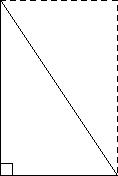
\includegraphics[scale=1]{pbpAreaRight.pdf}
\end{image}
\vfill
\end{problem}

\begin{problem}
``Shearing'' is a process where you take a shape, cut it into thin parallel strips, 
and then move the strips in a direction parallel to the strips to make a new shape.  
By Cavalieri's principle:\index{Cavalieri's principle}
\begin{quote}
Shearing parallel to a fixed direction does not change the $n$-dimensional measure of an object.
\end{quote}
What is this saying?
\vfill
\end{problem}

\newpage

\begin{problem}
Building on the first two problems, explain how the following picture
  ``proves'' that the area of any triangle is one half of the base times the
  height.
\begin{image}
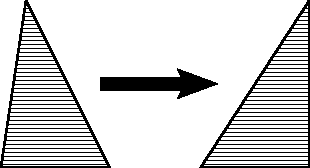
\includegraphics{pbpShearTri.pdf}
\end{image}
\vfill
\end{problem}

\begin{problem}
Explain how to use a picture to ``prove'' that a triangle of a given
  area could have an arbitrarily large perimeter.
\vfill
\end{problem}

\newpage

\begin{problem}
Shearing is a special case of Cavalieri's principle, which, in two dimensions, is stated as follows:  
\begin{quote}
Suppose two regions in a plane are contained between two parallel lines.  If every line parallel to the given lines intersects the two regions in equal lengths, then the regions have equal area.  
\end{quote}
Give an intuitive argument explaining why Cavalieri's principle is true.
\vfill
\end{problem}

\begin{problem}
State Cavalieri's principle in three dimensions.  
\vfill
\end{problem}

%
%\begin{problem}
%Sketch a net for a right pyramid of height $2''$ with a $2'' \times
%2''$ square base. Share your sketch with your neighbor---does it look
%OK?
%\end{problem}
%
%
%\begin{problem}
%Give detailed diagrams that show that a cube can be constructed from
%three equal pyramids.
%\end{problem}
\newpage

\begin{problem}
Cut out the provided net.  Then fold it and tape it to create a square-based pyramid.  With your neighbors, show that three such square-based pyramids can form a cube.  
\begin{image}
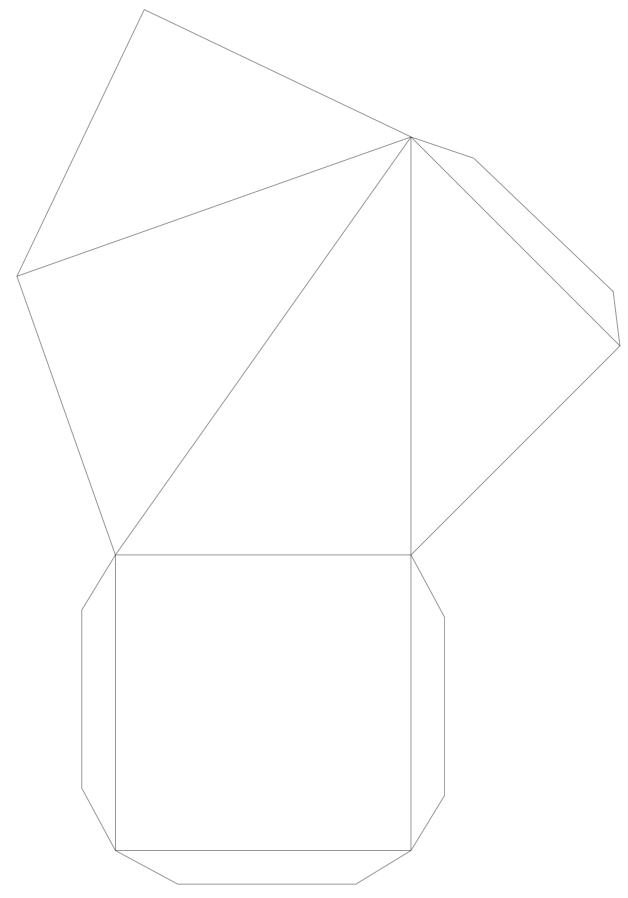
\includegraphics[scale=1.1]{rightPyramid}
\end{image}
\end{problem}

\newpage
\begin{problem}
Use your work above to derive a formula for the volume of a
right pyramid with a square base. The formula should be in terms of
the side length of the square base.
\vfill
\end{problem}

\begin{problem}
Use Cavalieri's principle to explain the formula for \textbf{every} pyramid with an $s\times s$ square base of height $s$ in terms of $s$.  Be sure to describe how this formula is different from the previous one.  
\vfill
\end{problem}

\begin{problem}
Provide an informal explanation of a volume formula for any pyramid-like object with a base of area $B$ and height $h$.  Be sure to describe what you mean by ``pyramid-like'' and whether your formula works for a cone.  
\vfill
\end{problem}

%\margincomment{CCSS G-GMD.1. Give an informal argument for the formulas for the
%  circumference of a circle, area of a circle, volume of a cylinder,
%  pyramid, and cone. \clarification{Use dissection arguments, Cavalieri's principle,
%  and informal limit arguments.}}
%  
%\margincomment{CCSS 8.G.9. Know the formulas for the volumes of cones, cylinders, and
%  spheres and use them to solve real-world and mathematical
%  problems.}

\newpage

\begin{problem}
In this problem you derive the formula for the volume of a sphere of 
radius $r$.\margincomment{CCSS G-GME.2. Give an informal argument using Cavalieri's principle for the formulas for the volume of a sphere and other solid figures.}
The figures below shows a half-sphere of radius $r$ alongside a cylinder of radius $r$ and height $r$ with a cone of radius $r$ and height $r$ removed.
\begin{image}\resizebox{.4\textwidth}{!}{%
    \begin{tikzpicture}
      \clip (-3.2,-2) rectangle (3.2,4);
  %% back of base
  \begin{scope} 
  \clip (-3,-2) rectangle (4,3);
  \draw (0,0) ellipse (3cm and .5cm);
  \end{scope}
  
  %% front of base
  \begin{scope} 
  \clip (-3.3,0) rectangle (3.3,-3);
  \draw[ultra thick] (0,0) ellipse (3cm and .5cm);
  \end{scope}

  %% Mid ellipse
  \draw[fill=black!20!white] (0,1.5) ellipse (2.6cm and .5cm);

  %% triangle
  \draw[thick,rounded corners=.5] (0,0) -- (0,1.5) -- (2.6,1.5) -- cycle;

  
  %% dome
  \draw[ultra thick] (3,0) arc (0:180:3);

  
  %% labels
  \node[left] at (0,.75) {$h$};
  \node[above] at (1.3,1.5) {$s$};
  \node[right] at (1.4,.75) {$r$};
  \end{tikzpicture}}
  \resizebox{.4\textwidth}{!}{\begin{tikzpicture}
      \clip (-3.2,-2) rectangle (4,4);
  %% back of base
  \begin{scope} 
  \clip (-3,0) rectangle (3,6);
  \draw (0,0) ellipse (3cm and .5cm);
  \end{scope}
  
  %% front of base
  \begin{scope} 
  \clip (-3.3,0) rectangle (3.3,-3);
  \draw[ultra thick] (0,0) ellipse (3cm and .5cm);
  \end{scope}

  %% top
  \draw[ultra thick] (0,3) ellipse (3cm and .5cm);

  
  %% outer cone (behind ellipse)
  \draw (0,0) -- (-1.5,1.5);
  \draw (0,0) -- (1.5,1.5);
  
  %% Mid ellipse
  \draw[fill=black!20!white] (0,1.5) ellipse (3cm and .5cm);
  \draw[fill=white] (0,1.5) ellipse (1.5cm and .25cm);

  %% outer cone (front of ellipse)
  \draw (-3,3) -- (-1.5,1.5);
  \draw (3,3) -- (1.5,1.5);
  

  %% sides
  \draw[ultra thick] (-3,0) -- (-3,3);
  \draw[ultra thick] (3,0) -- (3,3);


  
  %% labeled lengths
  %\draw[thick] (0,0) -- (0,1.5);
  \draw[thick] (-1.5,1.5) -- (0,1.5);
  \draw[thick] (0,0) -- (3,0);

  %% side brace
  \draw [decorate,decoration={brace,mirror},xshift=4pt,yshift=0pt]
(3,0) -- (3,1.5) node [black,midway,xshift=9pt] {$h$};

  %% labels
  %\node[left] at (0,.75) {$h$};
  \node[above] at (-.75,1.5) {$h$};
  \node[below] at (1.5,0) {$r$};
\end{tikzpicture}}
\end{image}
Think of $r$ as fixed, and think of $h$ as the varying height of a cross section.  The (hard to read) $s$ is the radius of the cross section of the sphere.  
\begin{enumerate}
\item The heights of the cylinder and the cone are not $h$.  What are their heights?  
\item What is $h$?  Explain why the several values labeled $h$ are indeed equal.   
\item Draw and label an ``aerial view'' of the cross sections.   
\item Explain why the cross sections at height $h$ have the same area.  
\item Use the formula for the volume of a cone and Cavalieri's principle to derive a formula for the volume of a sphere of radius $r$.  
\end{enumerate}
\vfill
\end{problem}

\end{document}
